\subsection{Acidity} \label{sensors:acidity}

As mentioned in the Design Report, the DFRobot SEN0169 V2 Pro \cite{SEN0169V2} was chosen for measuring the acidity. The manufacturer claims the sensor has a resolution of 0.1pH across the whole range from 0 to 14pH.\\

The chosen sensor was compared against the Hanna pHep, that also has a resolution of 0.1pH. \cite{hanna} Two solutions with different pH were tested on both sensors

\begin{figure}[h]
  \centering
  \begin{minipage}[b]{0.4\textwidth}
    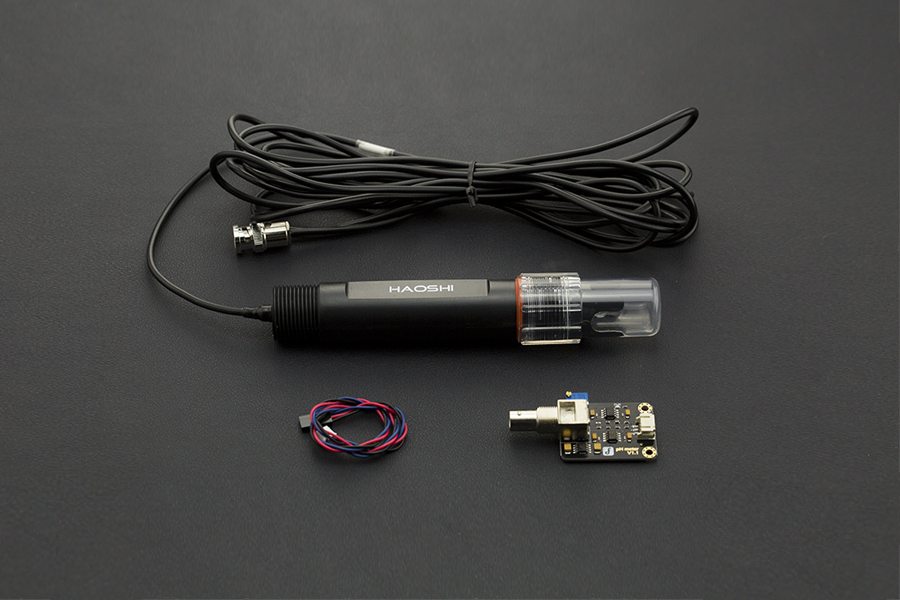
\includegraphics[width=\textwidth]{sensors/12_gravityv2pro.jpg}
    \caption{SEN0169 V2 Pro \cite{SEN0169V2}}
  \end{minipage}
  \hfill
  \begin{minipage}[b]{0.3\textwidth}
    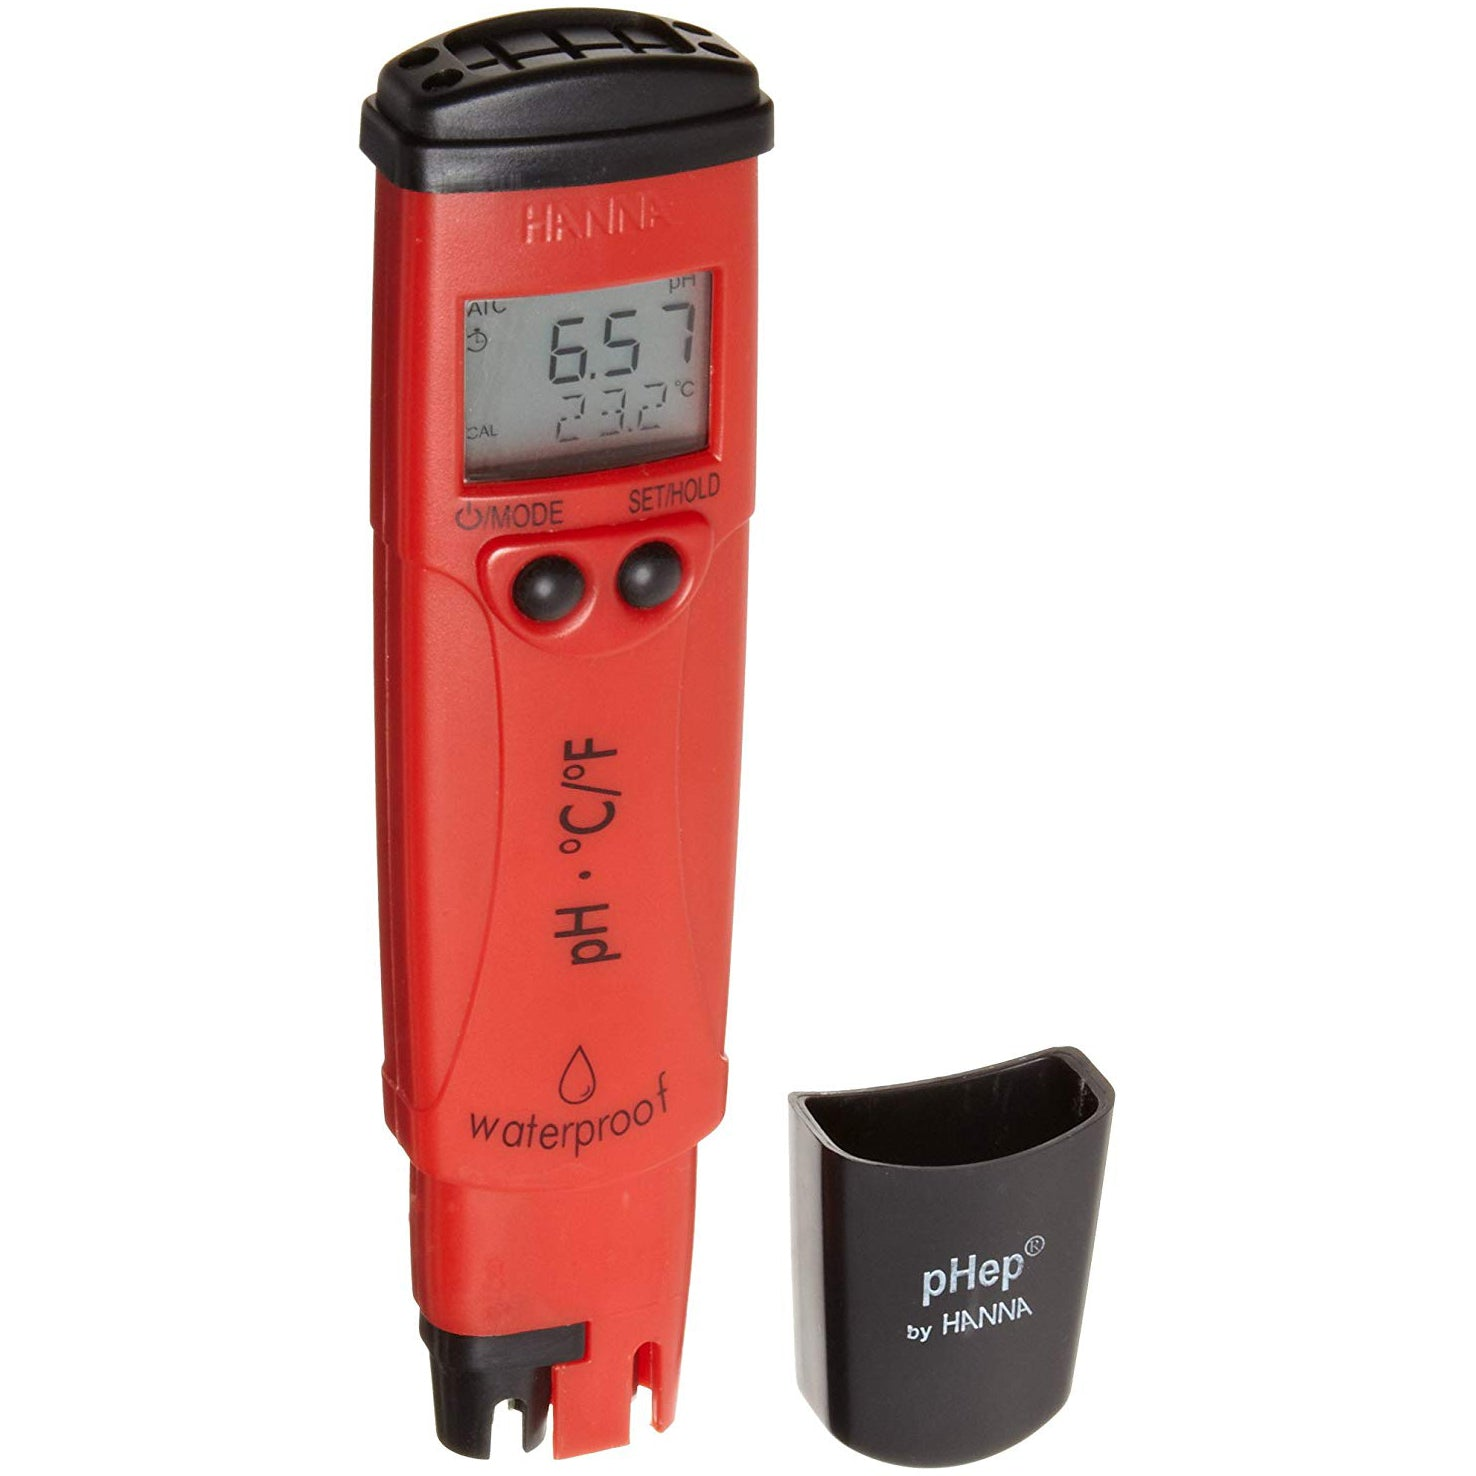
\includegraphics[width=\textwidth]{sensors/11_hanna.jpg}
    \caption{Hanna pHep \cite{hanna}}
  \end{minipage}
\end{figure}

\subsubsection{First solution}
The first solution is marked in pink. Both sensors repeatedly measured a pH of 4.4.

\begin{figure}[h]
  \centering
  \begin{minipage}[b]{0.2\textwidth}
    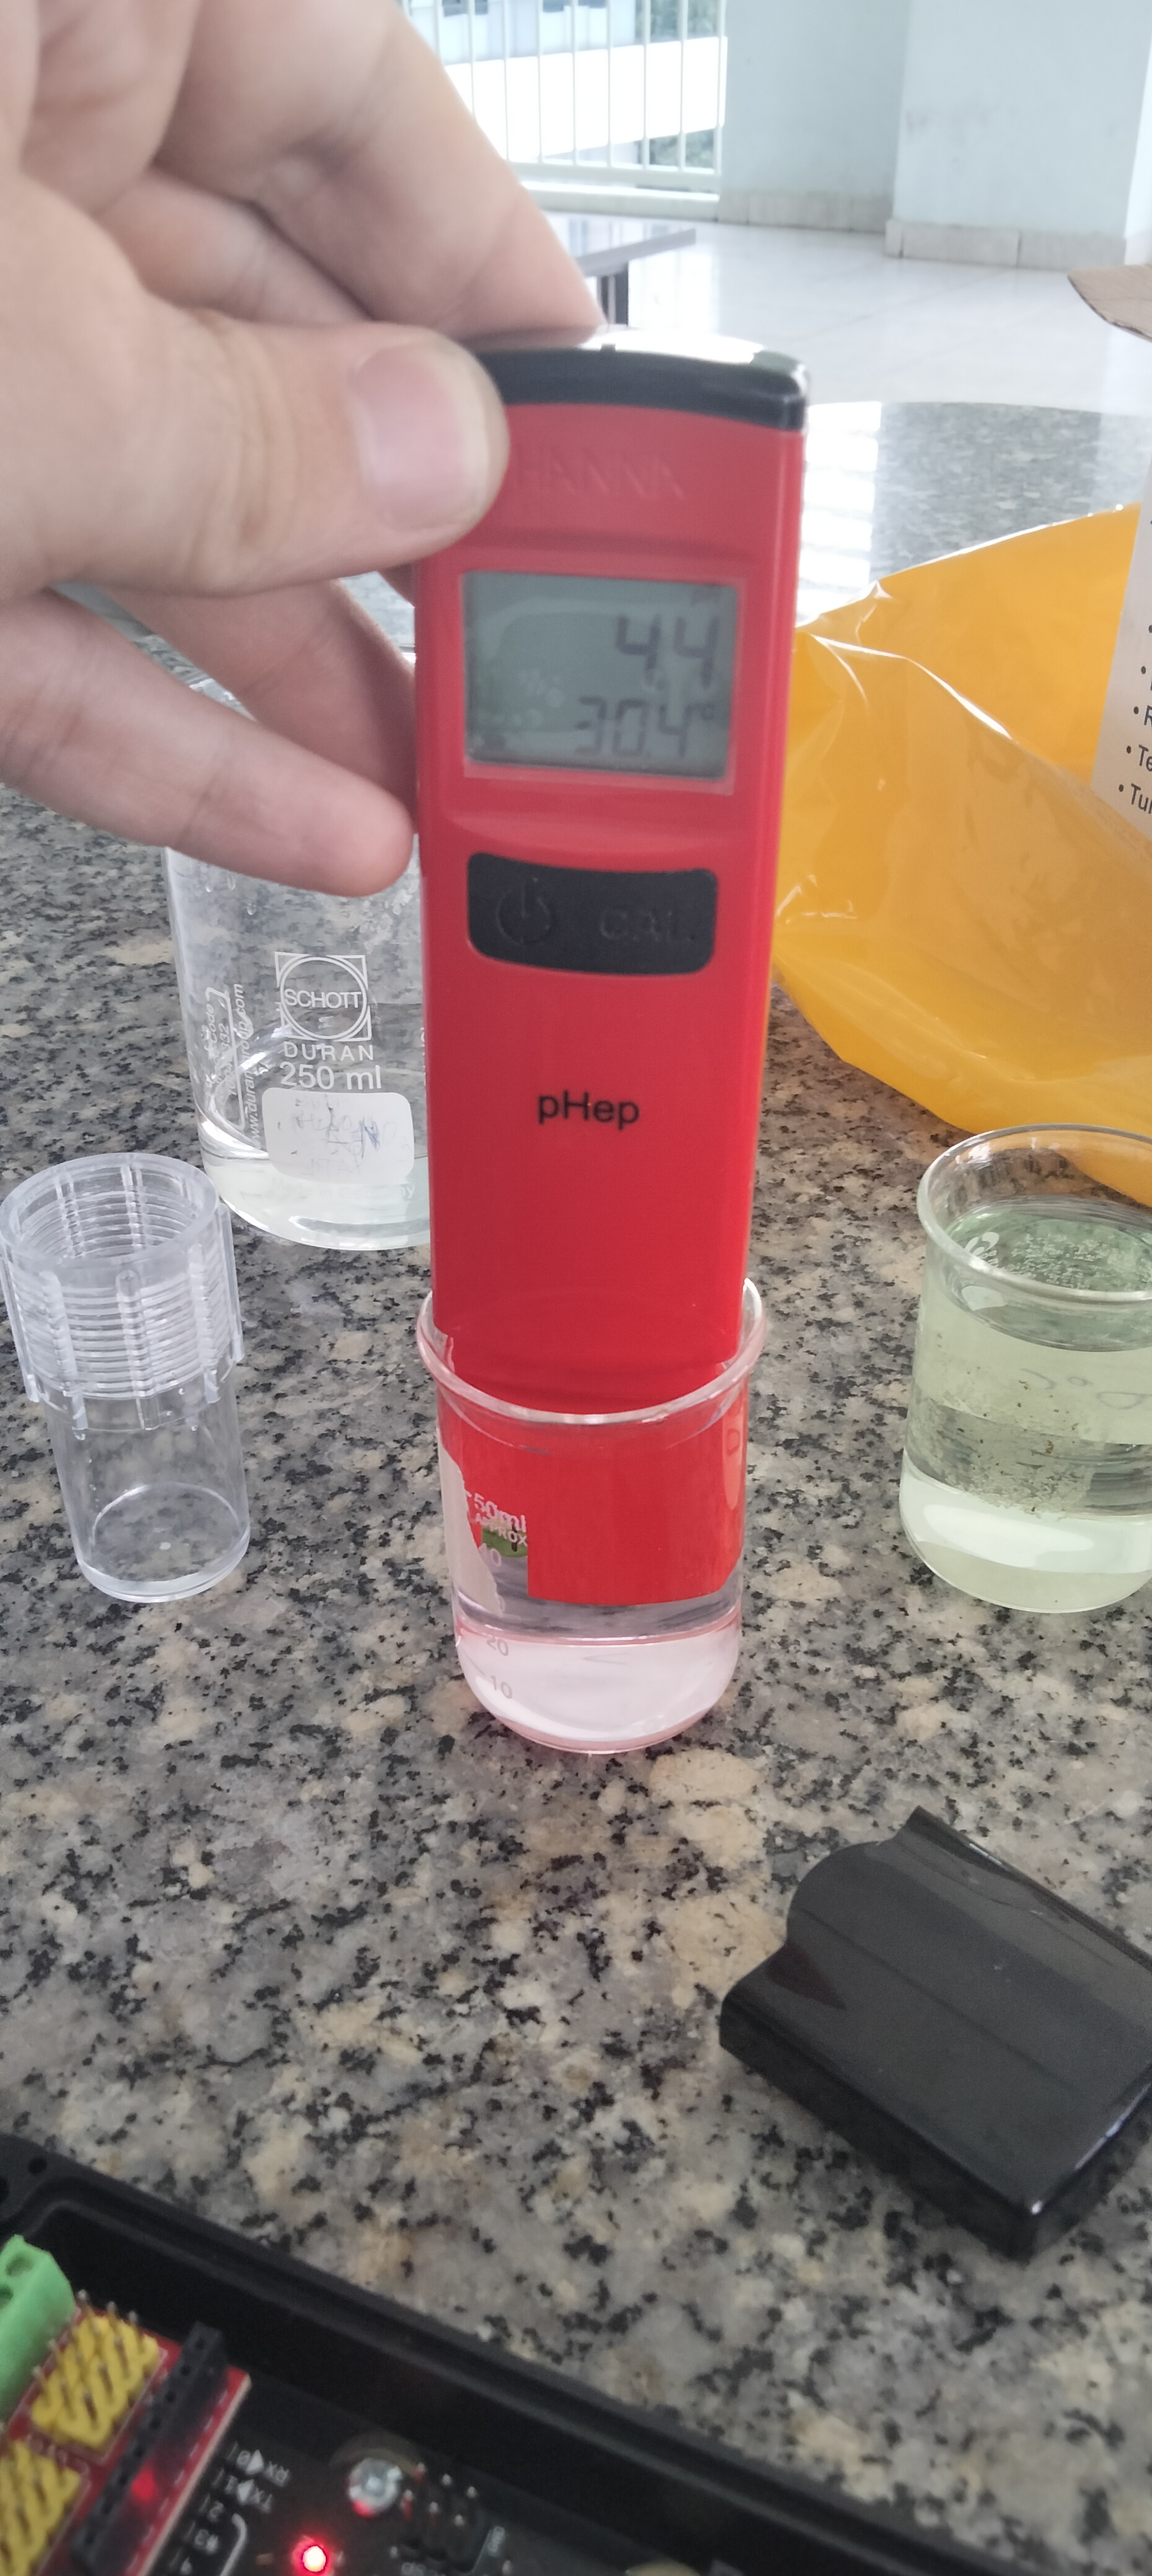
\includegraphics[width=\textwidth]{sensors/14_ph4_hanna.jpg}
    \caption{Hanna sensor measuring 4.4}
  \end{minipage}
  \hfill
  \begin{minipage}[b]{0.7\textwidth}
    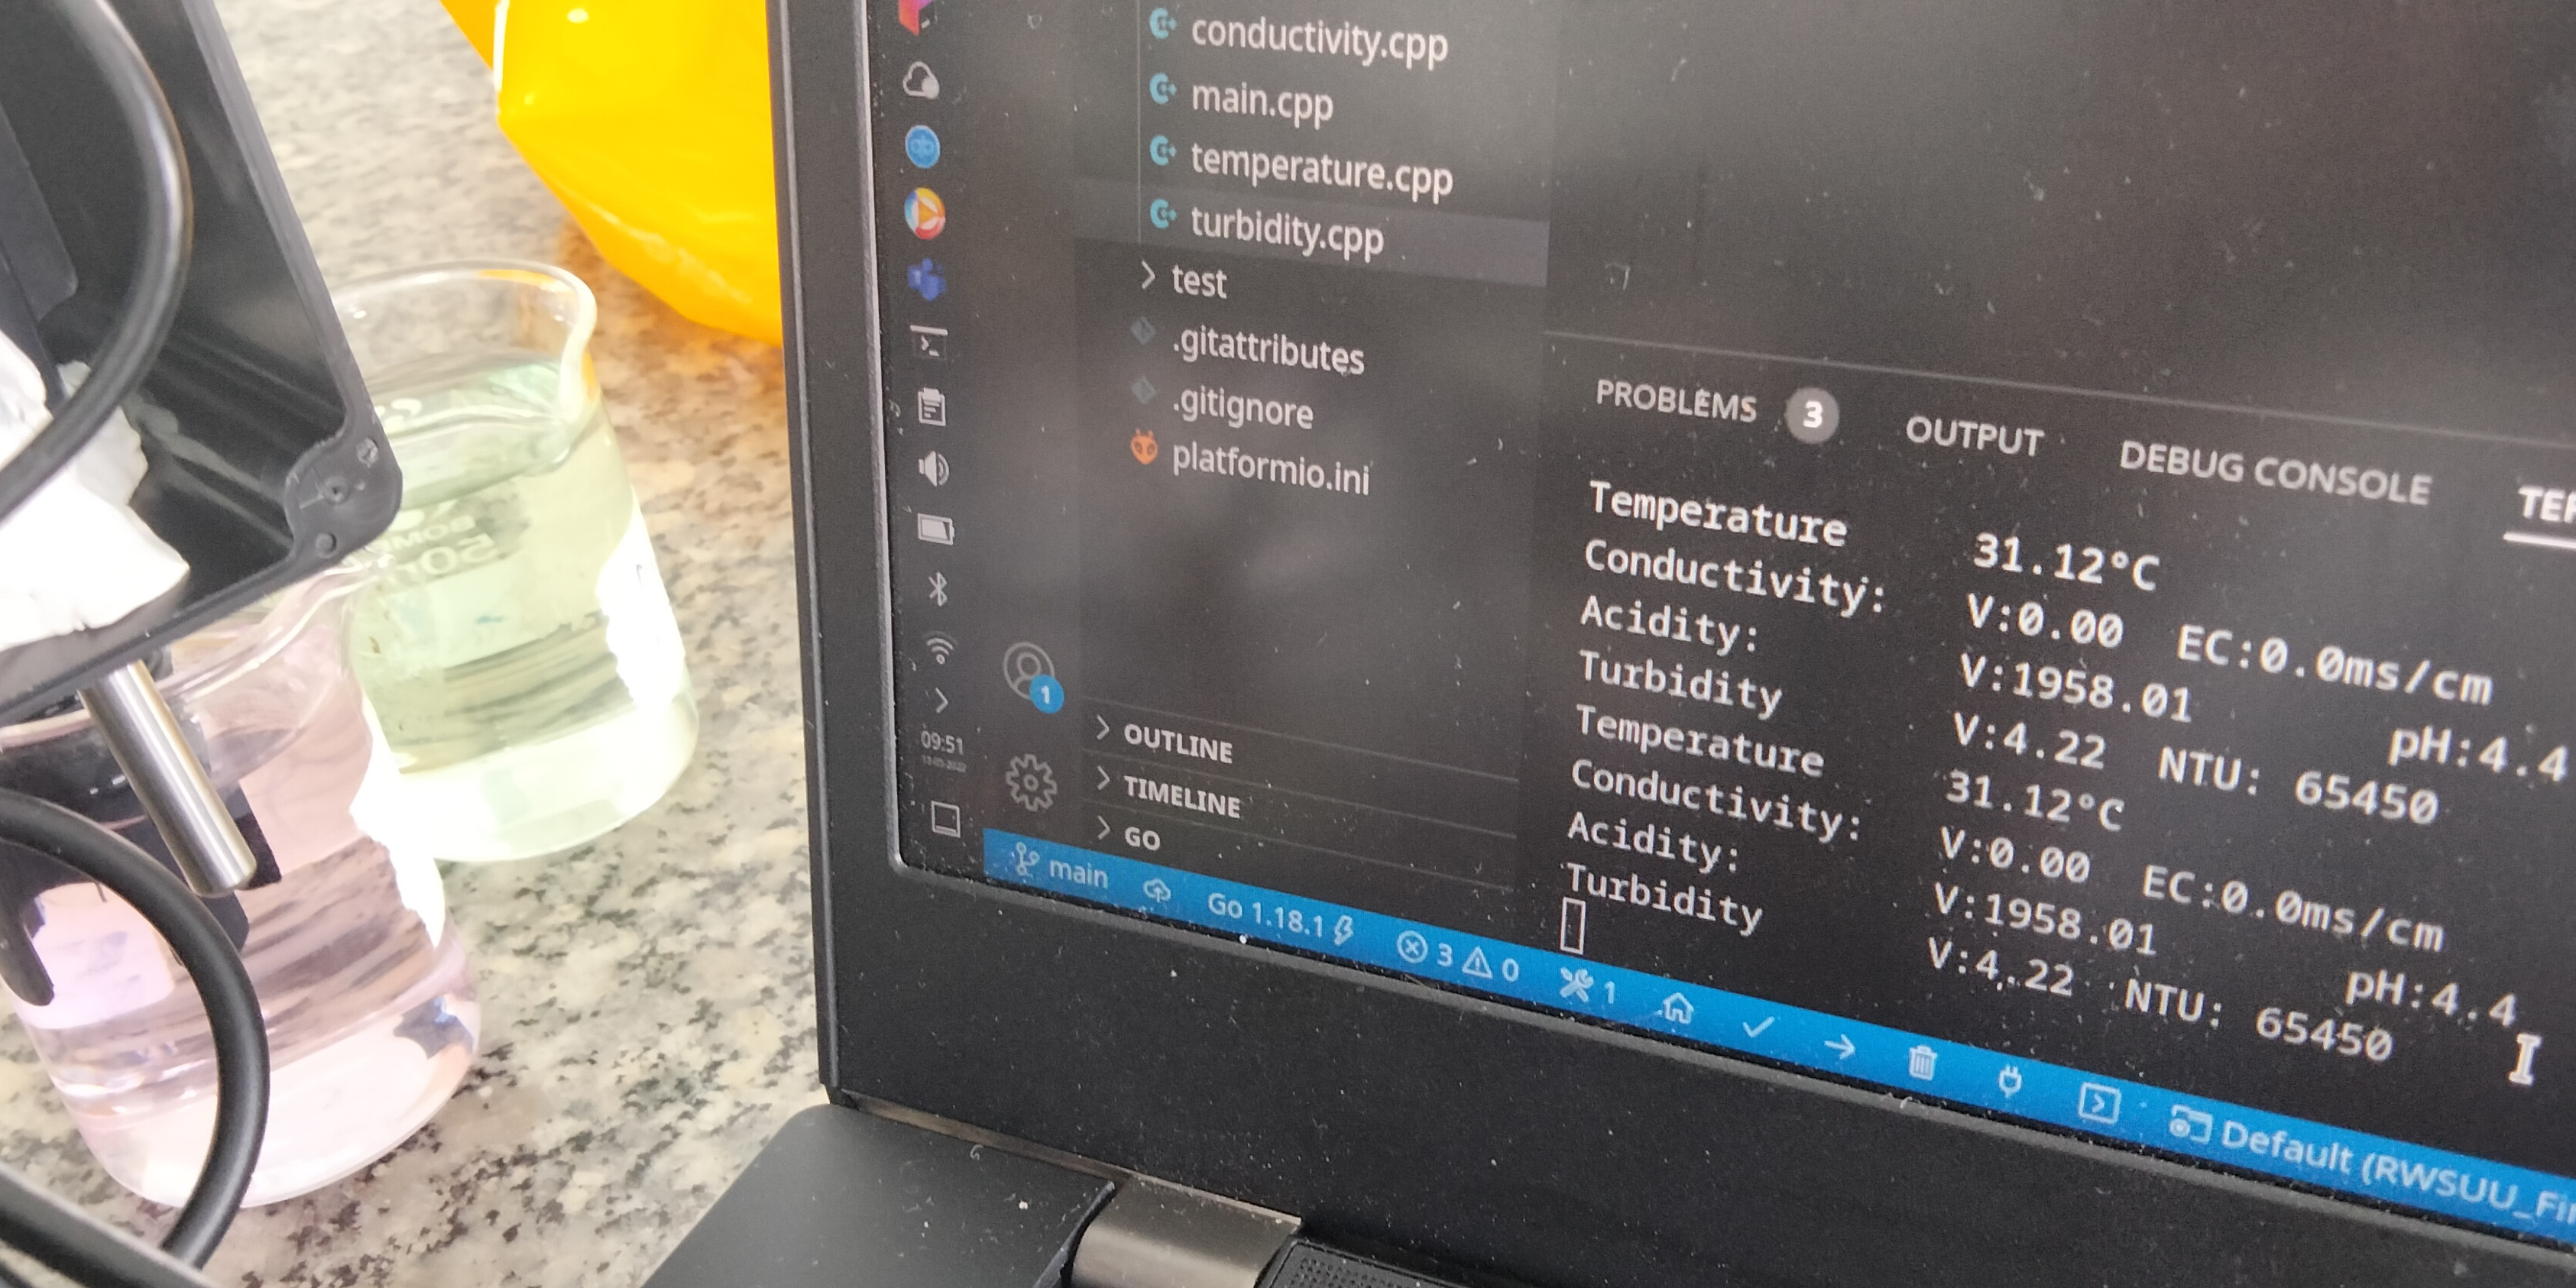
\includegraphics[width=\textwidth]{sensors/13_ph4_dfrobot.jpg}
    \caption{DFRobot sensor measuring 4.4}
  \end{minipage}
\end{figure}

\subsubsection{Second solution}
The second solution is marked in light yellow. The Hanna pHep repeatedly measured a pH of 7.2, while the DFRobot sensor repeatedly measured a pH of 7.3

\begin{figure}[h]
  \centering
  \begin{minipage}[b]{0.2\textwidth}
    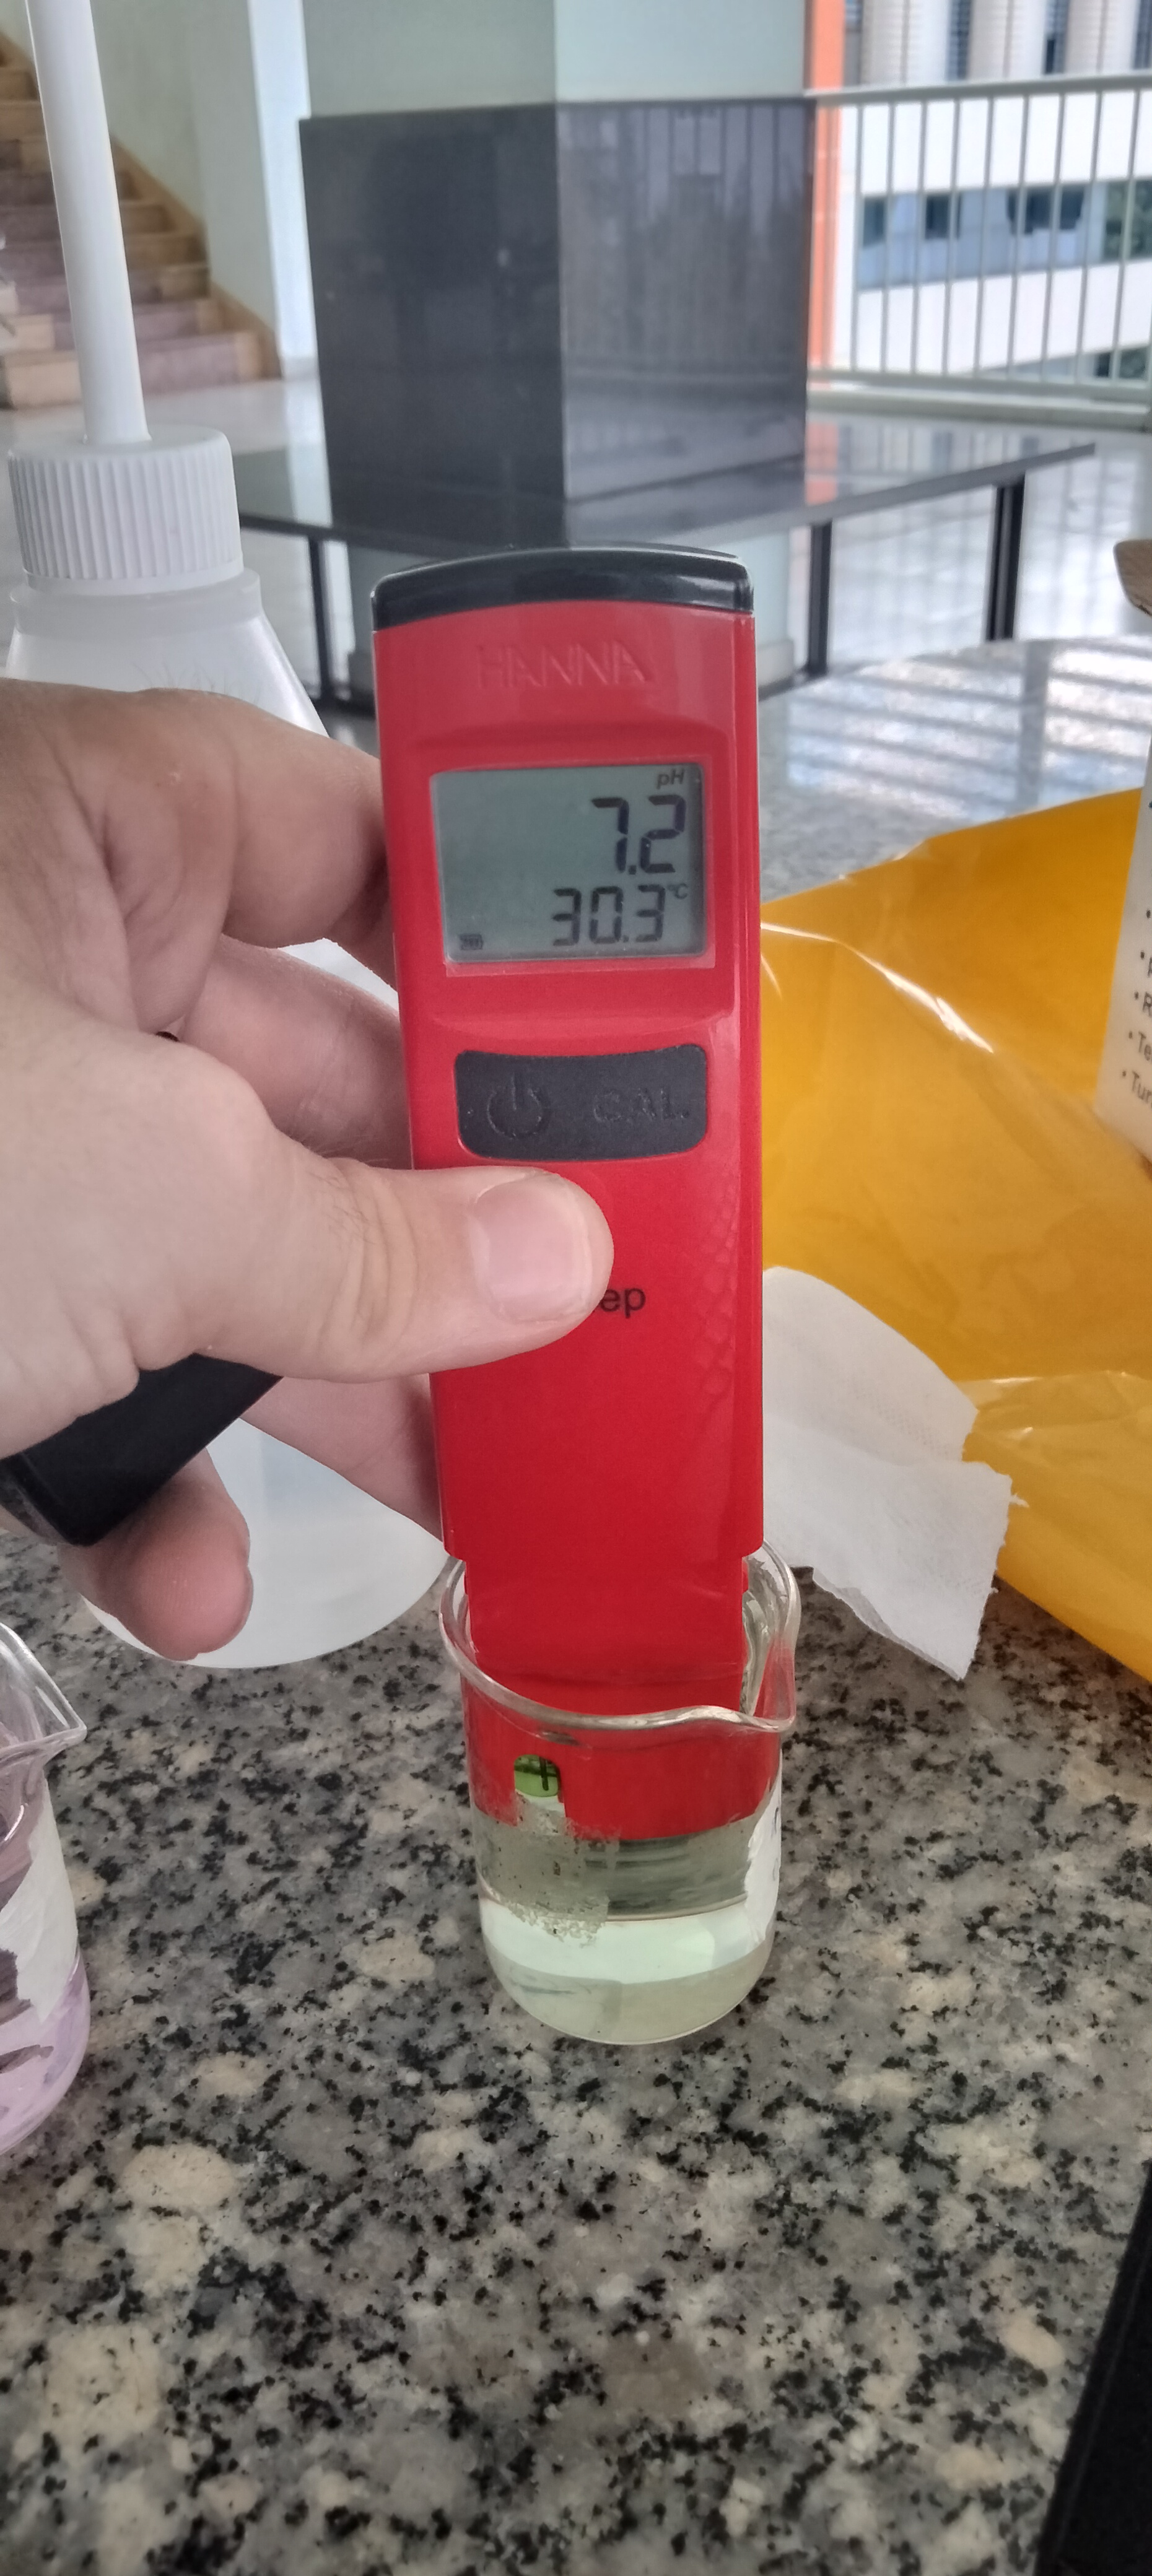
\includegraphics[width=\textwidth]{sensors/16_ph7_hanna.jpg}
    \caption{Hanna sensor measuring 7.2}
  \end{minipage}
  \hfill
  \begin{minipage}[b]{0.7\textwidth}
    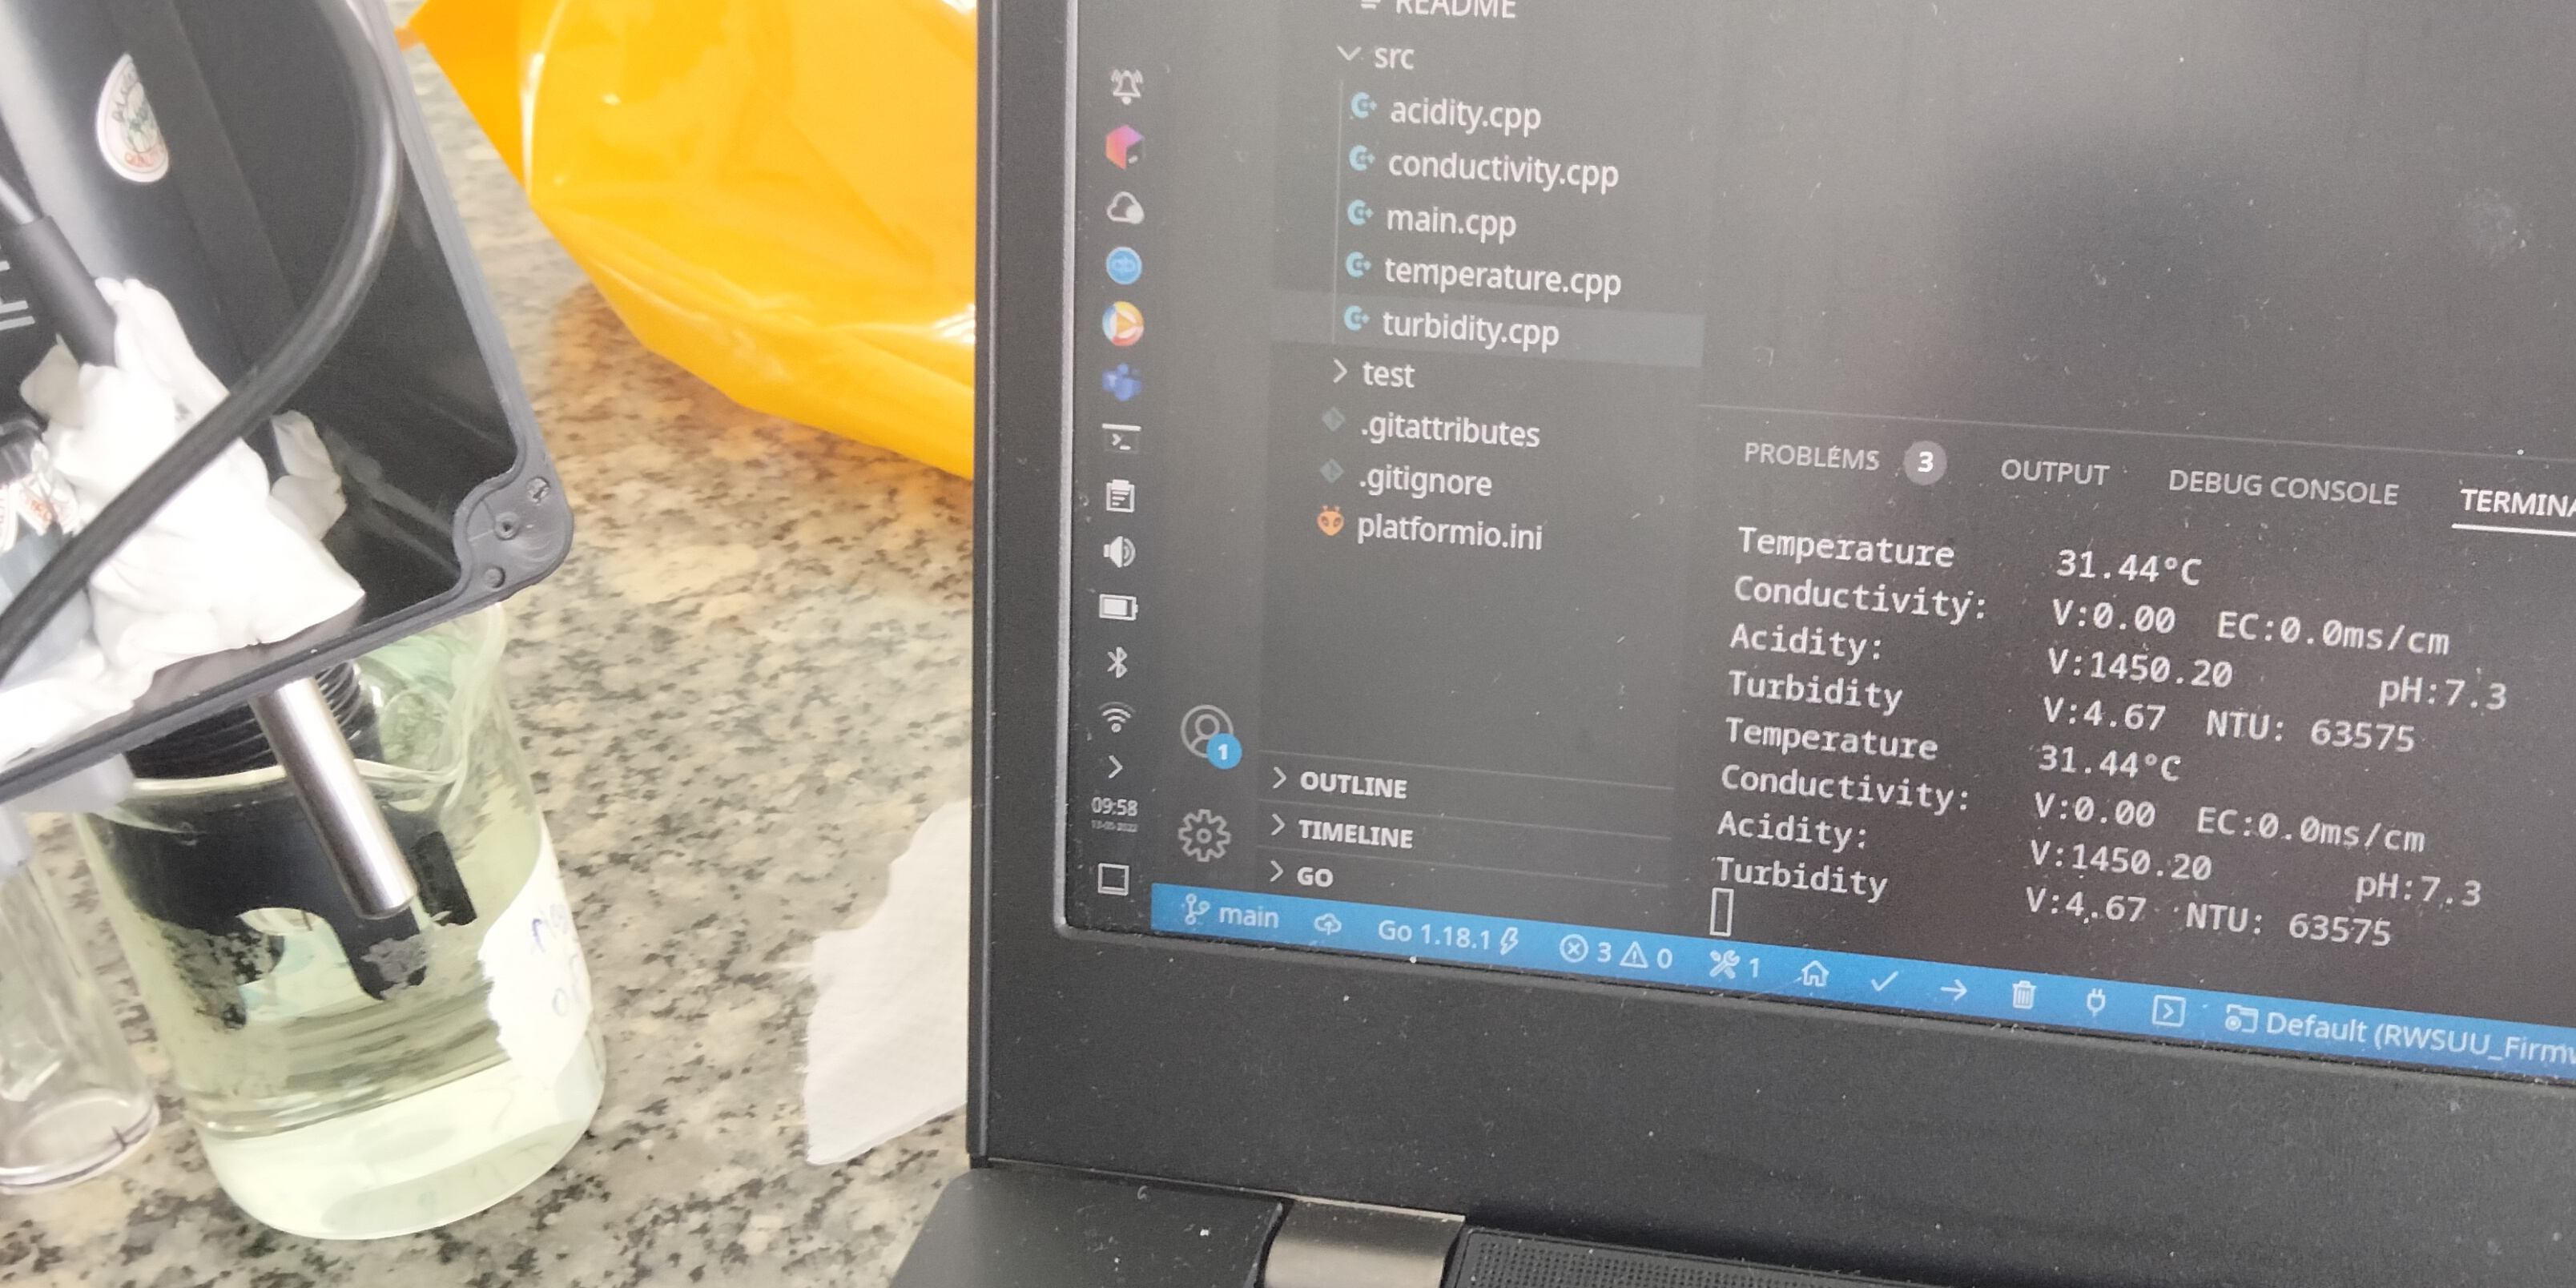
\includegraphics[width=\textwidth]{sensors/15_ph7_dfrobot.jpg}
    \caption{DFRobot sensor measuring 7.3}
  \end{minipage}
\end{figure}
